\documentclass[12pt]{article}
\usepackage{mathtools,amssymb}
\usepackage[margin=.65in]{geometry}
\usepackage[dvipsnames]{xcolor}
\usepackage{mathptmx}
\usepackage{pifont} % for wingdings and whatnot
\usepackage{tabularx}
\usepackage{parskip}
\usepackage{booktabs}
\usepackage{tikz}
\usetikzlibrary{angles,quotes} %angles for pic, quotes for ease of labeling pic
\usetikzlibrary{decorations.pathreplacing}% allows for bracket labeling
\tikzset{mypoint/.style={draw,fill,circle,minimum size=4pt,inner sep=0pt},
myhollowpoint/.style={draw,circle,minimum size=4pt,inner sep=0pt}}
\graphicspath{{media/}}
\usepackage{enumitem}
% To help with aligning item letters and numerals:
\SetLabelAlign{Center}{\makebox[1em]{\hfil\!#1\!\!\!\hfil})}
\usepackage[colorlinks=true, urlcolor=blue]{hyperref}
\pagestyle{empty}

%\everymath{\displaystyle}

% groovy underlining
\usepackage[normalem]{ulem}
\usepackage{contour}
\renewcommand{\ULdepth}{1.8pt}
\contourlength{0.8pt}
\newcommand{\myuline}[1]{%
  \uline{\phantom{#1}}%
  \llap{\contour{white}{#1}}%
}

% all minipage raggedright
\makeatletter
\let\@minipagerestore=\raggedright
\makeatother

% custom commands, envirnments, lists and column types
\newcommand{\blank}[1]{\underline{\hspace{#1}}} % \blank{30mm} creates a 30mm underlined blank

\newcolumntype{L}[1]{>{\raggedright\let\newline\\\arraybackslash\hspace{0pt}}m{#1}}
\newcolumntype{C}[1]{>{\centering\let\newline\\\arraybackslash\hspace{0pt}}m{#1}}
\newcolumntype{R}[1]{>{\raggedleft\let\newline\\\arraybackslash\hspace{0pt}}m{#1}}

\newcommand{\myfrac}[3][1pt]{%\genfrac{<ldelim>}{<rdelim>}{<thickness>}{<mathmode>}{<num>}{<denom>}
    \genfrac{}{}{}{}{\raisebox{#1}{$#2$}}{\raisebox{-#1-3pt}{$#3$}}}

% used to bold a row in a table
\newcolumntype{+}{>{\global\let\currentrowstyle\relax}}
\newcolumntype{^}{>{\currentrowstyle}}
\newcommand{\rowstyle}[1]{\gdef\currentrowstyle{#1} %
#1\ignorespaces
}

% set custom header/footer
\usepackage{titlesec}
\titleformat{\section}{\huge\bfseries}{\thesection}{1em}{}
\titleformat{\subsection}{\LARGE\bfseries}{\thesubsection}{1em}{}

\usepackage{titleps} % alternative to fncyhdr
\newpagestyle{main}{%
  \setheadrule{1pt} %
  \sethead{}{}{\thesubsection~\subsectiontitle}% \sethead{<left>}{<centre>}{<right>}
  \setfoot{}{}{Page \thepage}% \setfoot{<left>}{<centre>}{<right>}
}
\pagestyle{main}


\begin{document}
\raggedright

\section{Latex Reference}

\thispagestyle{empty}







\subsection{For Tests, Worksheets, and Notes}
\addcontentsline{toc}{subsection}{Power and Root Laws}

\begin{center}
\fbox{
\begin{minipage}{.9\textwidth}
\setlength{\abovedisplayskip}{1ex}
\setlength{\belowdisplayskip}{-2ex}
%\setlength{\abovedisplayshortskip}{0ex}
%\setlength{\belowdisplayshortskip}{0ex}
\medskip
A {\bfseries linear function} is a function of the form
\[
f(x) = mx + b
\]
\medskip
\end{minipage}
}
\end{center}


\begin{enumerate}
\item Find the $\text{n}^\text{\em th}$ dimension of the universe.

\begin{enumerate}[label=\alph*, align=Center]
\begin{tabular}[t]{ @{} b{75mm} b{80mm} @{} }
\item 42 &
\item the size of an atom \\[3ex]
\end{tabular}\\
\begin{tabular}[t]{ @{} b{140mm} @{} }
\item ``Money makes money. And the money that makes money makes money.'' \\
\mbox{}\hfill--Benjamin Franklin \\[3ex]
\item stuff \\
\item more stuff
\end{tabular}
\newline
\begin{minipage}[t]{.75\textwidth}
\vspace{0pt}
\item \leavevmode\vadjust{\vspace{-\baselineskip}}\newline
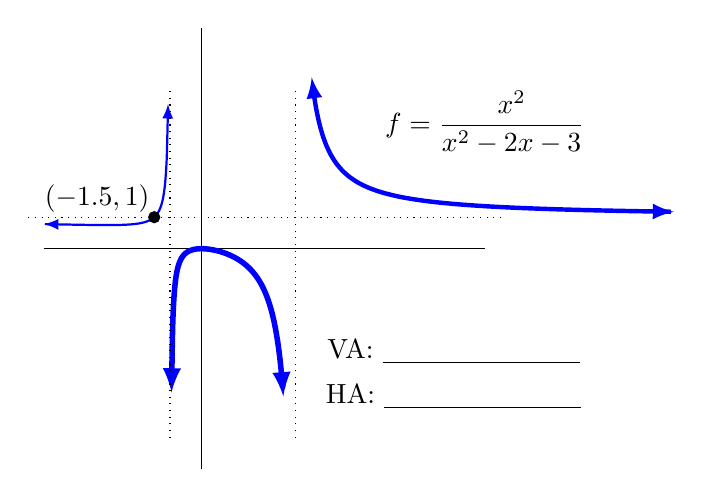
\begin{tikzpicture}[scale=.4]
\draw (-5,0) -- (9,0) (0,-7) -- (0,7);
\draw[blue,thick,latex-latex,smooth,samples=100,domain=-5:-1.06] plot(\x,{(\x)^(2)/((\x)^(2)-2*\x-3)});
\draw[blue,line width=2pt,latex-latex,smooth,samples=100,domain=-.95:2.6] plot(\x,{(\x)^(2)/((\x)^(2)-2*\x-3)});
\draw[blue,ultra thick,latex-latex,smooth,samples=100,domain=3.5:15] plot(\x,{(\x)^(2)/((\x)^(2)-2*\x-3)});
\draw[dotted] (-5.5,1) -- (9.5,1) (-1,-6) -- (-1,5) (3,-6) -- (3,5);
\node at (8,-4)[align=center]{VA: \blank{25mm} \\[1ex] HA: \blank{25mm}};
\node at (9,4){\normalsize$f=\dfrac{x^2}{x^2-2x-3}$};
\node[mypoint,label={[inner sep=0pt,fill=white,rectangle]135:{$(-1.5,1)$}}] at (-1.5,1){};
\end{tikzpicture}
\hfill
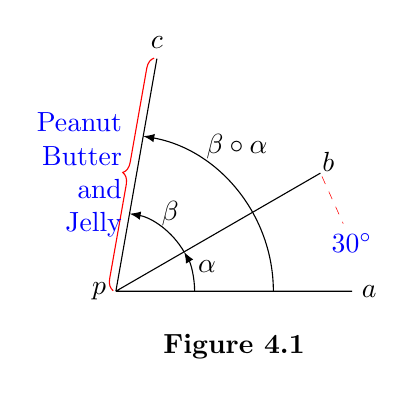
\begin{tikzpicture}
\coordinate (p) at (0,0);
\coordinate (a) at (0:3);
\coordinate (b) at (30:3);
\coordinate (c) at (80:3);
\node at (p)[left]{$p$};
\node at (a)[right]{$a$};
\node at (b)[above right=-1mm]{$b$};
\node at (c)[above]{$c$};
\draw (p) -- (a)
(p) -- (b)
(p) -- (c);
\pic [draw, -latex, "$\alpha$"{xshift=0mm,yshift=0mm}, angle eccentricity=1.2, angle radius = 1cm] {angle = a--p--b};
\pic [draw, -latex, "$\beta$"{xshift=0mm,yshift=0mm}, angle eccentricity=1.2, angle radius = 1cm] {angle = b--p--c};
\pic [draw, -latex, "$\beta\circ\alpha$"{xshift=-3mm,yshift=3mm}, angle eccentricity=1.2, angle radius = 2cm] {angle = a--p--c};
\node at (1.5,-.7){\bfseries Figure 4.1};
\node[inner sep=1pt,pin={[pin distance=6mm,pin edge={red,dashed}]270,blue,xshift=4mm:{$30^\circ$}}] at (b){};
\draw [red,decoration={brace,amplitude=4pt,raise=1pt,mirror},decorate] (c) -- node[left=0.4ex,align=right,blue] {Peanut\\Butter\\and\\Jelly} (p);
\end{tikzpicture}
\end{minipage}
\end{enumerate}
\end{enumerate}

\hrulefill


\begin{minipage}[t]{.45\textwidth}
\vspace{0pt}
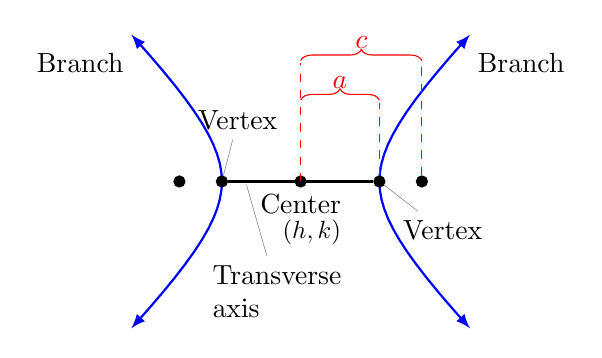
\begin{tikzpicture}
% eccentricity setup
\pgfmathsetmacro{\e}{1.4}   % eccentricity
    \pgfmathsetmacro{\a}{1}
    \pgfmathsetmacro{\b}{(\a*sqrt((\e)^2-1)}
    \draw[domain=-1.4:1.4,blue,thick,latex-latex] plot ({\a*cosh(\x)},{\b*sinh(\x)});
    \draw[domain=-1.4:1.4,blue,thick,latex-latex] plot ({-\a*cosh(\x)},{\b*sinh(\x)});
% points on transverse axis
\path (-1.54,0) node[mypoint](f1){}
 -- (-1,0) node[mypoint,pin={90,xshift=2mm}:Vertex](v1){}
 -- (0,0) node[mypoint,label={[label distance=-1pt]below,align=right:Center \\ \raisebox{1mm}{\scalebox{.9}{$(h,k)$}}}](center){}
 -- (1,0) node[mypoint,pin={315,xshift=-2mm}:Vertex](v2){}
 -- (1.54,0) node[mypoint](f2){};
% draw and label transverse axis segment
\draw[thick] (v1) -- (v2);
\node[inner sep=1pt,pin={[pin distance=9mm]270,xshift=4mm,align=left:{Transverse \\ axis}}] at (-.7,0){};
% label branches
\node at (-2.8,1.5) {Branch};
\node at (2.8,1.5) {Branch};
% dimensioning center to vertex a and focus c
\coordinate (a1) at (0,1); % left end of a bracket
\coordinate (a2) at (1,1); % right end of a bracket
\coordinate (c1) at (0,1.5); % left end of c bracket
\coordinate (c2) at (1.54,1.5); % right end of c bracket
\draw [red,dashed] (0,0) -- (c1);
\draw [red,dashed] (f2) -- (c2);
\draw [red,dashed] (v2) -- (a2);
\draw [red,decoration={brace,amplitude=4pt,raise=1pt}, decorate] (a1) -- node[above=0.4ex] {$a$} (a2);
\draw [red,decoration={brace,amplitude=4pt,raise=1pt}, decorate] (c1) -- node[above=0.4ex] {$c$} (c2);
\end{tikzpicture}
\end{minipage}
\begin{minipage}[t]{.45\textwidth}
\vspace{0pt}
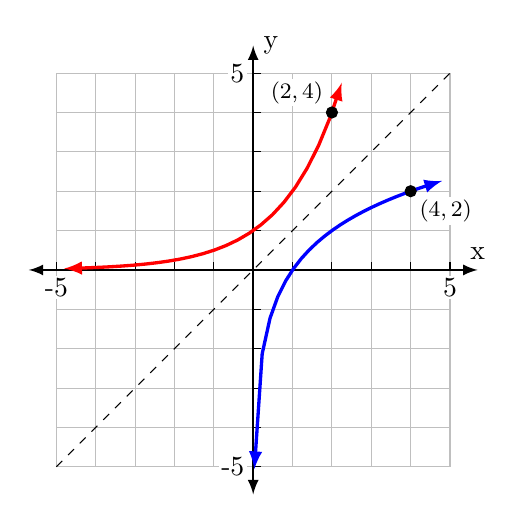
\begin{tikzpicture}[scale=.5]
\draw[lightgray] (-5,-5) grid (5,5);
\draw [thick,latex-latex] (-5.7,0) -- (5.7,0) node[above]{\normalsize x};
\foreach \xtick in {-5,...,5}{
\draw (\xtick,.2) -- (\xtick,0);
}
\foreach \xlabel in {-5,5}{
\node at (\xlabel,0)[below=2pt,fill=white,inner sep=1pt]{\xlabel};
}

\draw [thick,latex-latex] (0,-5.7) -- (0,5.7) node[right]{\normalsize y};
\foreach \ytick in {-5,...,5}{
\draw (.2,\ytick) -- (0,\ytick);
}
\foreach \ylabel in {-5,5}{
\node at (0,\ylabel)[left=2pt,fill=white,inner sep=1pt]{\ylabel};
}

\draw[blue,very thick,latex-latex,domain=.03:4.8] plot (\x,{log2(\x)});
\draw[red,very thick,latex-latex,domain=-4.8:2.25] plot (\x,{2^(\x)});
\draw[dashed] (-5,-5) -- (5,5);
\node[mypoint] at (4,2){};
\draw (4,2) node[fill=white,rectangle,inner sep=1pt,anchor=north west,xshift=2pt,yshift=-2pt]{\footnotesize$(4,2)$};
\node[mypoint] at (2,4){};
\draw (2,4) node[fill=white,rectangle,inner sep=1pt,anchor=south east,xshift=-2pt,yshift=2pt]{\footnotesize$(2,4)$};
\end{tikzpicture}
\end{minipage}






%\pagebreak
%\clearpage
\newpage





\begin{minipage}{.55\textwidth}

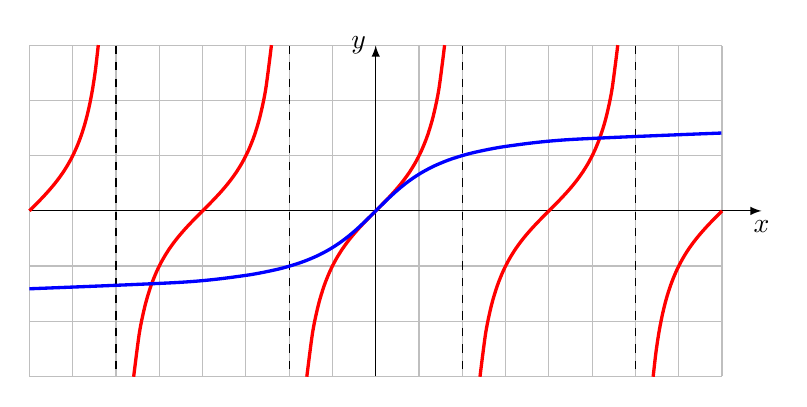
\begin{tikzpicture}[scale=.7]
\draw[lightgray,xstep=pi/4] (-2*pi,-3) grid (2*pi,3);
\draw[-latex] (-2*pi,0) -- (7,0)node[below]{$x$};
\draw[-latex] (0,-3) -- (0,3)node[left]{$y$};
\foreach \x in {-3/2*pi,-pi/2,pi/2,3/2*pi}
\draw[dashed] (\x,3) -- (\x,-3);

\foreach \i in {-pi,0,pi}
\draw[red,very thick,smooth,domain=-1.25-\i:1.25-\i] plot (\x,{tan(deg(\x))});
\draw[red,very thick,smooth,domain=-2*pi:-2*pi+1.25] plot (\x,{tan(deg(\x))});
\draw[red,very thick,smooth,domain=2*pi-1.25:2*pi] plot (\x,{tan(deg(\x))});
\draw[blue,very thick,smooth,domain=-1.413:1.413,xscale=-1,rotate=90] plot (\x,{tan(deg(\x))});
\end{tikzpicture}

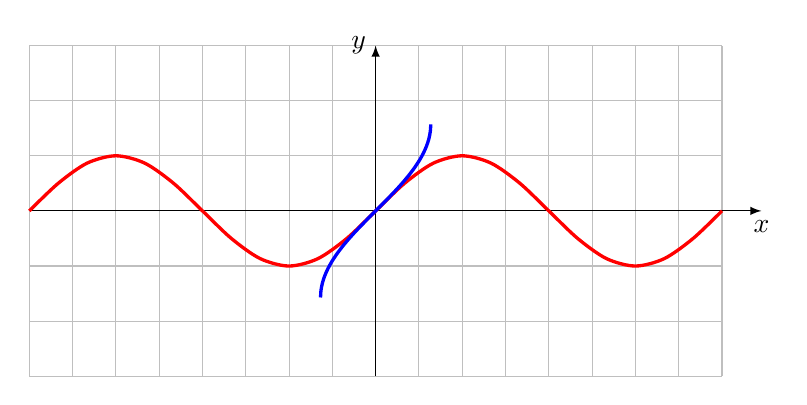
\begin{tikzpicture}[scale=.7]
\draw[lightgray,xstep=pi/4] (-2*pi,-3) grid (2*pi,3);
\draw[-latex] (-2*pi,0) -- (7,0)node[below]{$x$};
\draw[-latex] (0,-3) -- (0,3)node[left]{$y$};
\draw[red,very thick,smooth,domain=-2*pi:2*pi] plot (\x,{sin(deg(\x))});
\draw[blue,very thick,smooth,domain=-pi/2:pi/2,xscale=-1,rotate=90] plot (\x,{sin(deg(\x))});
\end{tikzpicture}

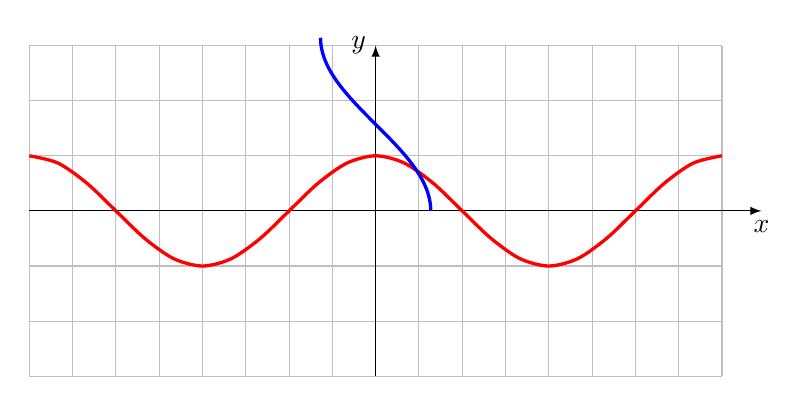
\begin{tikzpicture}[scale=.7]
\draw[lightgray,xstep=pi/4] (-2*pi,-3) grid (2*pi,3);
\draw[-latex] (-2*pi,0) -- (7,0)node[below]{$x$};
\draw[-latex] (0,-3) -- (0,3)node[left]{$y$};
\draw[red,very thick,smooth,domain=-2*pi:2*pi] plot (\x,{cos(deg(\x))});
\draw[blue,very thick,smooth,domain=0:pi,xscale=-1,rotate=90] plot (\x,{cos(deg(\x))});
\end{tikzpicture}
\end{minipage}
\hfill
\begin{minipage}{.4\textwidth}
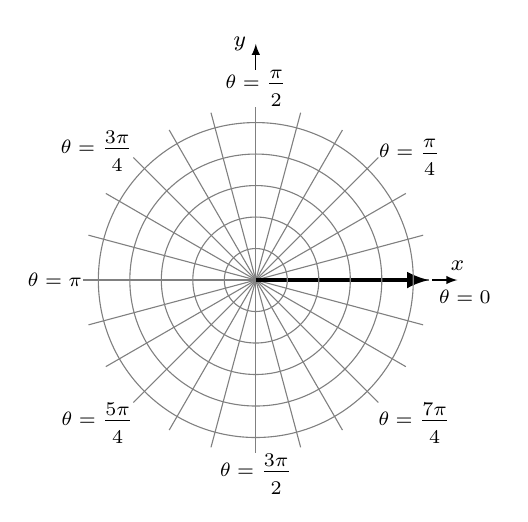
\begin{tikzpicture}[scale=.4,nodes={font=\scriptsize}]
\def\myrad{5} %number of circles (should scale entire plot)
\draw[-latex] (0,0) --(0:\myrad+1.4) node[above]{\footnotesize$x$};
\draw[-latex] (0,0) -- (90:\myrad+2.5) node[left]{\footnotesize$y$};
\draw[white] (0,0) -- (0:\myrad+.6);
\draw[white] (0,0) -- (90:6.6);
\foreach \t in {0,15,30,45,60,75,90,105,120,135,150,165,180,195,210,225,240,255,270,285,300,315,330,345}
\draw[gray] (0,0) -- (\t:\myrad+.5) coordinate (\t);
\draw[-latex,line width=.6mm] (0,0) --(0:\myrad+.5);
\foreach \r in {1,...,\myrad}
\draw[gray] (0,0) circle (\r);
\node at (0)[below right]{$\theta = 0$};
\node at (45)[anchor=180,inner sep=0pt]{$\theta=\myfrac{\pi}{4}$};
\node at (90)[anchor=270,inner sep=0pt,fill=white]{$\theta=\myfrac{\pi}{2}$};
\node at (135)[anchor=350,inner sep=0pt]{$\theta=\myfrac{3\pi}{4}$};
\node at (180)[anchor=0,inner sep=0pt]{$\theta=\pi$};
\node at (225)[anchor=30,inner sep=0pt]{$\theta=\myfrac{5\pi}{4}$};
\node at (270)[anchor=90,inner sep=0pt,fill=white]{$\theta=\myfrac{3\pi}{2}$};
\node at (315)[anchor=150,inner sep=0pt]{$\theta=\myfrac{7\pi}{4}$};
\end{tikzpicture}


\def\centx{3}
\def\centy{0}
\def\radi{2}
\begin{tikzpicture}
\draw[-latex] (-0.5,0) -- (5.5,0) node[below]{$x$};
\draw[-latex] (0,-2.5) -- (0,2.5) node[left]{$y$};
\shade[ball color = gray!40, opacity = 0.4] (\centx,\centy) circle (\radi cm);
\draw (\centx,\centy) circle (\radi cm);
\draw (\centx-\radi,\centy) arc (180:360:{\radi} and 0.6);
\draw[dashed] (\centx+\radi,\centy) arc (0:180:{\radi} and 0.6);
\end{tikzpicture}
\end{minipage}


\fbox{
\begin{minipage}{.97\textwidth}
\medskip
{\large\bfseries Finding the Volume of a Solid of Revolution by Slicing}\par\bigskip
\begin{description}[leftmargin=!,labelwidth=\widthof{Step 1. },itemsep=1ex]
\item[Step 1.] Sketch the plane region that is to be revolved, finding the points of intersection of bounding curves.
\item[Step 2.] On the sketch, draw a typical think rectangle perpendicular to the axis of revolution, that is, either perpendicular to the $x$-axis and of width $\Delta x$ or perpendicular to the $y$-axis and of width $\Delta y$.
\item[Step 3.] {\em Looking at the sketch}, write down the volume $V_\text{slice}$ of the slice swept out as the rectangle is revolved about the given axis.  Express $V_\text{slice}$ entirely in terms of the variable ($x$ or $y$) appearing in the $\Delta$-increment.
\item[Step 4.] Integrate between the appropriate ($x$ or $y$) limits.  (Geometrically, this amounts to adding the volumes found in step 3 and taking the limit of the resulting sum as $||$.(
\end{description}
\medskip
\end{minipage}
}
\par\bigskip





\newpage









\textbf{True/False. Fill in the blank with T for true or F for false.}

\medskip

\begin{enumerate}
\begin{tabular}[t]{ @{} b{85mm} b{85mm} @{} }
\item \; \underline{\hspace{1cm}} \; $a^{\log_a{M}} = M$ &
\item \; \underline{\hspace{1cm}} \; $\log_a{a}^r = r$ \\[7mm]
\item \; \underline{\hspace{1cm}} \; $\log_a(MN) = \log_a{M} + \log_a{N}$ &
\item \; \underline{\hspace{1cm}} \; $\log_a\left(\dfrac{M}{N}\right) = \log_a{M} + \log_a{N}$ \\[9mm]
\item \; \underline{\hspace{1cm}} \; If $M=N$, then $\log_a{M} = \log_a{N}$ &
\item \; \underline{\hspace{1cm}} \; $\log_a{M}^r = r\log_a{M}$ \\[15mm]
\end{tabular}
\end{enumerate}






\begin{figure}[h!]
\centering
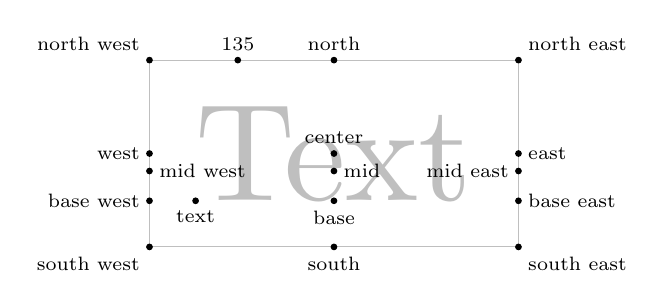
\begin{tikzpicture}
\node (mytext) [draw,lightgray,scale=5] at (0,0) {Text};

\tikzstyle{every node}=[font=\scriptsize]

\filldraw

(mytext.north west) [xshift=1pt,yshift=-1pt] circle (1pt) node[above left] {north west}
(mytext.north east) [xshift=-1pt,yshift=-1pt] circle (1pt) node[above right] {north east}
(mytext.south east) [xshift=-1pt,yshift=1pt] circle (1pt) node[below right] {south east}
(mytext.south west) [xshift=1pt,yshift=1pt] circle (1pt) node[below left] {south west}

(mytext.north) [yshift=-1pt] circle (1pt) node[above] {north}
(mytext.south) [yshift=1pt] circle (1pt) node[below] {south}
(mytext.east) [xshift=-1pt] circle (1pt) node[right] {east}
(mytext.west) [xshift=1pt] circle (1pt) node[left] {west}

(mytext.mid east) [xshift=-1pt] circle (1pt) node[left] {mid east}
(mytext.mid west) [xshift=1pt] circle (1pt) node[right] {mid west}

(mytext.base east) [xshift=-1pt] circle (1pt) node[right] {base east}
(mytext.base west) [xshift=1pt] circle (1pt) node[left] {base west}

(mytext.center) circle (1pt) node[above] {center}
(mytext.mid) circle (1pt) node[right] {mid}
(mytext.base) circle (1pt) node[below] {base}
(mytext.text) circle (1pt) node[below] {text}

(mytext.135) [yshift=-1pt] circle (1pt) node[above] {135};
\end{tikzpicture}
\end{figure}




\includegraphics[width=.4\textwidth]{Lenna.png}
\includegraphics[keepaspectratio, scale=.5, clip=true, trim=20mm 25mm 80mm 90mm ]{Lenna}

% Include entire pdf page(s):

% \usepackage{pdfpages}
% \includepdf[pages=-,pagecommand={},width=\textwidth]{file.pdf}






%\pagebreak
%\clearpage
\newpage













\subsection{A few more examples}
\addcontentsline{toc}{subsection}{A few More eXaMpLeS} %changes the TOC
\subsectionmark{a FEW more ExAmPlEs} %changes the header



\begin{figure}[h!]
\centering
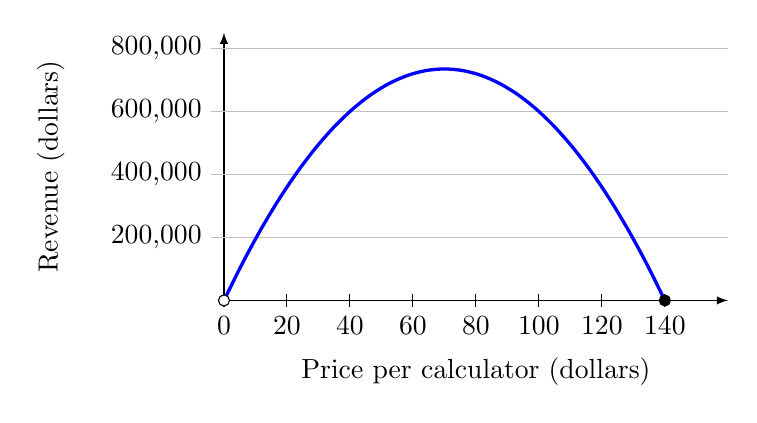
\begin{tikzpicture}[scale=.04]
\draw[-latex] (0,0) -- (160,0) node[midway,below=6mm]{Price per calculator (dollars)};
\draw[-latex] (0,0) -- (0,85) node[midway,xshift=-22mm,rotate=90]{Revenue (dollars)};
\foreach \x in {0,20,40,60,80,100,120,140}
\draw (\x,2) -- (\x,-2) node[below]{\x};
\foreach \y in {20,40,60,80}
\draw[lightgray] (160,\y) -- (-4,\y) node[left]{\textcolor{black}{\y0,000}};
\draw[blue,very thick,smooth,domain=0:140] plot (\x,{-.015*\x*\x + 2.1*\x});
\draw (0,0) node[mypoint,fill=white]{};
\draw (140,0) node[mypoint]{};
\end{tikzpicture}
\end{figure}



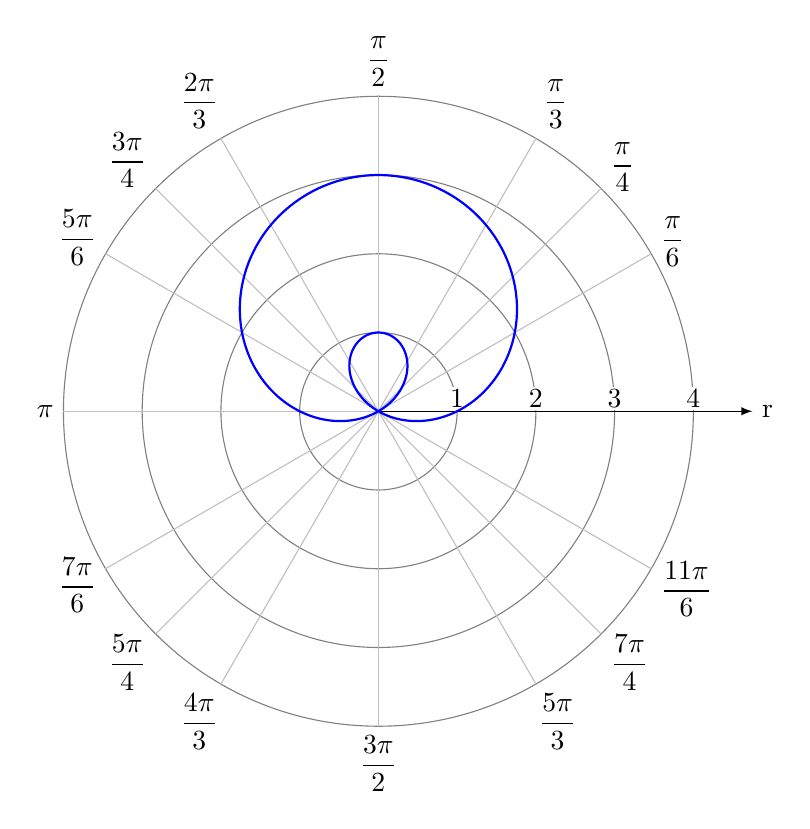
\begin{tikzpicture}[line cap=round,line join=round]
\foreach \x in {1,...,4} {
	\draw (0,0) [color=gray] circle [radius = \x];
}
\draw[-latex] (0,0) -- (4.75,0) node[right] {r};
\foreach \x in {1,...,4} { % polar axis marks and labels
	\draw[thick,shift={(\x,0)}] (0pt,-4pt) node[above=4pt,fill=white,inner sep=1pt] {$\x$};
}
\foreach \x/\t in {
30/$\dfrac{\pi}{6}$,
45/$\dfrac{\pi}{4}$,
60/$\dfrac{\pi}{3}$,
90/$\dfrac{\pi}{2}$,
120/$\dfrac{2\pi}{3}$,
135/$\dfrac{3\pi}{4}$,
150/$\dfrac{5\pi}{6}$,
180/$\pi$,
210/$\dfrac{7\pi}{6}$,
225/$\dfrac{5\pi}{4}$,
240/$\dfrac{4\pi}{3}$,
270/$\dfrac{3\pi}{2}$,
300/$\dfrac{5\pi}{3}$,
315/$\dfrac{7\pi}{4}$,
330/$\dfrac{11\pi}{6}$
} {
    \draw[lightgray] (0,0) -- (\x: 4) node[anchor=180+\x] {\color{black} \t};
}
\draw[domain=0:3*pi,samples=500,blue,thick] plot ({deg(\x)}:{1+2*sin(\x r)});
\end{tikzpicture}

\begin{tikzpicture}
\draw[-latex] (-3,0)--(3,0) node[below]{$x$};
\draw[-latex] (0,-3)--(0,3) node[right]{$y$};
\draw[thick,samples=200,domain=125:-35]plot(\x:{3*sin(\x)*cos(\x)/(sin(\x)^3+cos(\x)^3)});
\node[mypoint] at (3/2,3/2){};
\node[above right] at (3/2,3/2){$\left(\tfrac{3}{2},\tfrac{3}{2}\right)$};
\draw (1.5875,1.3) -- (1.5875,0) node[below]{$2^{2/3}$};
 \end{tikzpicture}




\newpage











\subsection{Tables}






\begin{tabular}{@{}+b{.18\textwidth}@{}^p{.45\textwidth}@{}^p{.37\textwidth}@{}} % see preamble for setup of bold row
\toprule\rowstyle{\bfseries}%
Environment & Code & Notes \\ \toprule
array             &
\verb|\begin{array}[pos]{cols}| \newline \verb| rows| \newline \verb|\end{array}| &
use in math mode \newline \verb|\usepackage{array}| \\ \midrule
tabular           &
\verb|\begin{tabular}[pos]{cols}| \newline \verb| rows| \newline \verb|\end{tabular}| &
use in text mode \newline \verb|\usepackage{array}| \\ \midrule
tabular*          &
\verb|\begin{tabular*}{width}[pos]{cols}| \newline \verb| rows| \newline \verb|\end{tabular*}| & \verb|width| is space between columns
\newline \verb|\usepackage{array}| \\ \midrule
tabularx          &
\verb|\begin{tabularx}{width}[pos]{cols}| \newline \verb| rows| \newline \verb|\end{tabularx}| & \verb|width| is total table width
\newline \verb|\usepackage{tabularx}| \newline tabularx loads the array package \\ \bottomrule
\end{tabular}



\begin{tabular}{+l^c^c^c}
\toprule\rowstyle{\bfseries}%
Quantity                     & Symbol  & Unit   & Value \\ \toprule %
Stiffness in $z$ direction   & $k_z$   & $N/m$  & 2276  \\ \midrule
Stiffness in $r$ direction   & $k_r$   & $N/m$  & 3414  \\ \midrule
Weight of the body           & $P$     & $N$    & 35    \\ \bottomrule
\end{tabular}

\bigskip

\begin{tabular}{>{\bfseries}lp{8cm}}
\toprule
Force & Force is a vector quantity defined as the rate of
change of the momentum of the body that would be induced by that
force acting alone. \\ \midrule
Moment of a force & Moment of a force
with respect to an origin is defined as the cross product of the
position vector (with respect to the same origin) and the
force. \\ \bottomrule
\end{tabular}

\bigskip

\begin{tabular*}{\textwidth}[tb]%
{>{\bfseries}l@{\extracolsep{\fill}}p{8cm}}
\toprule
Force & Force is a vector quantity defined as the rate of
change of the momentum of the body that would be induced by that
force acting alone. \\ \midrule
Moment of a force & Moment of a force
with respect to an origin is defined as the cross product of the
position vector (with respect to the same origin) and the
force. \\ \bottomrule
\end{tabular*}


\bigskip

\begin{tabularx}{\textwidth}{>{\bfseries}lX}
\toprule
Force & Force is a vector quantity defined as the rate of change of
the momentum of the body that would be induced by that
force acting alone. \\ \midrule
Moment of a force & Moment of a force with respect to an origin is
defined as the cross product of the position vector ( with respect to
the same origin ) and the
force. \\ \bottomrule
\end{tabularx}





\newpage





\subsection{Fonts, Size,
Tiny Bullets, and Underlining}
\myuline{\bfseries\large Groovy underlining and tiny bullets}


\renewcommand{\labelitemi}{$\vcenter{\hbox{\tiny$\bullet$}}$}
\begin{itemize}[nosep]
\item Tiny bullet size
\item for the discrete itemizer
\end{itemize}

\begin{table}[h!]
\centering
\begin{tabular}{ @{} p{.18\textwidth} @{} p{.15\textwidth} @{} p{.3\textwidth} @{} L{.37\textwidth} @{} }
Command & Switch & Font Styles & Description \\ \toprule
\ttfamily \textbackslash textnormal\{\} & \ttfamily\textbackslash normalfont & document font family & This is the default or normal font. \\ \midrule
\ttfamily \textbackslash emph\{\}       & \ttfamily\textbackslash em         &
\em emphasis & Typically italics.  Using emph\{\} inside of italic text removes the intalics on the emphasized text. \\ \midrule
\ttfamily \textbackslash textrm\{\}     & \ttfamily\textbackslash rmfamily   &
\rmfamily roman font family &  \\ \midrule
\ttfamily \textbackslash textsf\{\}     & \ttfamily\textbackslash sffamily   &
\sffamily sans serif font family &  \\ \midrule
\ttfamily \textbackslash texttt\{\}     & \ttfamily\textbackslash ttfamily   &
\ttfamily typewritter/teletype & This is a fixed-width or monospace font. \\ \midrule
\ttfamily \textbackslash textup\{\}     & \ttfamily\textbackslash upshape    &
\upshape upright shape & The same as the normal typeface. \\ \midrule
\ttfamily \textbackslash textit\{\}     & \ttfamily\textbackslash itshape    &
\itshape italic shape &  \\ \midrule
\ttfamily \textbackslash textsl\{\}     & \ttfamily\textbackslash slshape    &
\slshape slanted shape & Similar to, but slightly different from, italics. \\ \midrule
\ttfamily \textbackslash textsc\{\}     & \ttfamily\textbackslash scshape    &
\scshape Small Capitals &  \\ \midrule
\ttfamily \textbackslash uppercase\{\}  &                                    &
\uppercase{Uppercase(all caps)} &  \\ \midrule
\ttfamily \textbackslash textbf\{\}     & \ttfamily\textbackslash bfseries   &
\bfseries bold &  \\ \midrule
\ttfamily \textbackslash textmd\{\}     & \ttfamily\textbackslash mdseries   &
\mdseries medium weight & The normal font weight. \\ \midrule
\ttfamily \textbackslash lfseries\{\}   & \ttfamily\textbackslash lfseries   &
light & Not supported by all typefaces.  \\ \bottomrule
\end{tabular}
\end{table}


% this code requires no packages
{
\newcommand*{\alphabet}{abcdefghijklmnopqrstuvwxyz}
\makeatletter
\newcommand*{\showalphabetwidth}[2]{%
  \fontfamily{#1}\selectfont
  \settowidth{\@tempdima}{\alphabet}%
  \alphabet~-- width for #2 at 1\@ptsize pt: \the\@tempdima
}
\makeatother

\showalphabetwidth{cmr}{Computer Modern}\\
\showalphabetwidth{ptm}{Times New Roman}\\
\showalphabetwidth{ppl}{Palatino}
}







\newpage








\subsection{{\ttfamily pifont} Quick Reference}
\verb|\usepackage{pifont}|

\begin{table}[h!]
\centering
\begin{tabular}{ r *{10}{c} }
    & 0 & 1 & 2 & 3 & 4 & 5 & 6 & 7 & 8 & 9 \\
\hline &&&&&&&&&&\\[-2ex]
0   &&&&&&&&&&\\
10  &&&&&&&&&&\\
20  &&&&&&&&&&\\
30  &&&&\ding{33}&\ding{34}&\ding{35}&\ding{36}&\ding{37}&\ding{38}&\ding{39}\\
40  &\ding{40}&\ding{41}&\ding{42}&\ding{43}&\ding{44}&\ding{45}&\ding{46}&\ding{47}&\ding{48}&\ding{49}\\
50  &\ding{50}&\ding{51}&\ding{52}&\ding{53}&\ding{54}&\ding{55}&\ding{56}&\ding{57}&\ding{58}&\ding{59}\\
60  &\ding{60}&\ding{61}&\ding{62}&\ding{63}&\ding{64}&\ding{65}&\ding{66}&\ding{67}&\ding{68}&\ding{69}\\
70 &\ding{70}&\ding{71}&\ding{72}&\ding{73}&\ding{74}&\ding{75}&\ding{76}&\ding{77}&\ding{78}&\ding{79}\\
80 &\ding{80}&\ding{81}&\ding{82}&\ding{83}&\ding{84}&\ding{85}&\ding{86}&\ding{87}&\ding{88}&\ding{89}\\
90 &\ding{90}&\ding{91}&\ding{92}&\ding{93}&\ding{94}&\ding{95}&\ding{96}&\ding{97}&\ding{98}&\ding{99}\\
100 &\ding{100}&\ding{101}&\ding{102}&\ding{103}&\ding{104}&\ding{105}&\ding{106}&\ding{107}&\ding{108}&\ding{109}\\
110 &\ding{110}&\ding{111}&\ding{112}&\ding{113}&\ding{114}&\ding{115}&\ding{116}&\ding{117}&\ding{118}&\ding{119}\\
120 &\ding{120}&\ding{121}&\ding{122}&\ding{123}&\ding{124}&\ding{125}&\ding{126}&&&\\
130 &&&&&&&&&&\\
140 &&&&&&&&&&\\
150 &&&&&&&&&&\\
160 &\ding{160}&\ding{161}&\ding{162}&\ding{163}&\ding{164}&\ding{165}&\ding{166}&\ding{167}&\ding{168}&\ding{169}\\
170 &\ding{170}&\ding{171}&\ding{172}&\ding{173}&\ding{174}&\ding{175}&\ding{176}&\ding{177}&\ding{178}&\ding{179}\\
180 &\ding{180}&\ding{181}&\ding{182}&\ding{183}&\ding{184}&\ding{185}&\ding{186}&\ding{187}&\ding{188}&\ding{189}\\
190 &\ding{190}&\ding{191}&\ding{192}&\ding{193}&\ding{194}&\ding{195}&\ding{196}&\ding{197}&\ding{198}&\ding{199}\\
200 &\ding{200}&\ding{201}&\ding{202}&\ding{203}&\ding{204}&\ding{205}&\ding{206}&\ding{207}&\ding{208}&\ding{209}\\
210 &\ding{210}&\ding{211}&\ding{212}&\ding{213}&\ding{214}&\ding{215}&\ding{216}&\ding{217}&\ding{218}&\ding{219}\\
220 &\ding{220}&\ding{221}&\ding{222}&\ding{223}&\ding{224}&\ding{225}&\ding{226}&\ding{227}&\ding{228}&\ding{229}\\
230 &\ding{230}&\ding{231}&\ding{232}&\ding{233}&\ding{234}&\ding{235}&\ding{236}&\ding{237}&\ding{238}&\ding{239}\\
240 &\ding{240}&\ding{241}&\ding{242}&\ding{243}&\ding{244}&\ding{245}&\ding{246}&\ding{247}&\ding{248}&\ding{249}\\
250 &\ding{250}&\ding{251}&\ding{252}&\ding{253}&\ding{254}&&&&&\\
\end{tabular}
\end{table}








\newpage









\subsection{Awesome discussions and interweb pages}
\begin{itemize}
\item \href{https://en.wikibooks.org/wiki/LaTeX/Lengths}{lengths in \LaTeX}
\item \href{https://tex.stackexchange.com/questions/71172/why-are-default-latex-margins-so-big}{margin length}
\item \href{https://www.overleaf.com/learn/latex/Page_size_and_margins}{page sizes and margins}
\item \href{http://www.texdoc.net/texmf-dist/doc/latex/geometry/geometry.pdf}{the geometry package documentation}
\item \href{https://www.overleaf.com/learn/latex/Writing_your_own_package}{writing your own package}
\item \href{https://www.overleaf.com/learn/latex/Writing_your_own_class}{writing your own class}
\item \href{https://www.latex-project.org/help/documentation/clsguide.pdf}{intro for class and package writers}
\item \href{http://tutex.tug.org/pracjourn/2005-4/hefferon/hefferon.pdf}{good (and simple?) example of writing a class}
\item \href{http://ptgmedia.pearsoncmg.com/images/9780201362992/samplepages/0201362996.pdf}{The \LaTeX Companion, Second Edition}
\item \href{https://www.ee.iitb.ac.in/~trivedi/LatexHelp/latexfont.htm}{detailed font help}
\item \href{https://alexwlchan.net/2017/10/latex-underlines/}{awesome underlining}
\item \href{https://www.tug.org/pracjourn/2007-1/mori/mori.pdf}{awesome guide to tables}
\end{itemize}







\end{document}